\documentclass[12pt,a4paper]{article}
\usepackage[utf8]{inputenc}
\usepackage[magyar]{babel}
\usepackage{amsmath}
\usepackage{amsfonts}
\usepackage{amssymb}
\usepackage{graphicx}
\usepackage[left=2cm,right=2cm,top=2cm,bottom=2cm]{geometry}

\sloppy
\frenchspacing

\author{Fülöp Endre}
\title{Data-flow elemzés gráfredukcióval}

\begin{document}

\maketitle

\section{Beveztés}
A fordításidejű program-analízis segítséget nyújt a fordítóprogramok által generált kód működésének vizsgálatához és optimalizálásához. Az analízis során a fordítóprogram megvizsgálja a program köztes reprezentációját, majd lehetőségeket keres olyan átalakításokra, melyek következtében a program valamilyen szempontból jobban teljesít futás közben. Ez lehet futásidő csökkenése, kisebb memóriahasználat, vagy akár optimális cache használat is. Az ilyen transzformációk esetében azonban fontos, hogy a program megőrizze eredeti jelentését is, vagyis az optimalizálónak érvelnie kell tudni arról, hogy a megkísérelt átalakítás biztonságos, szemantikailag azonos jelentésű kódhoz vezet.

Ebben az esszében bemutatom a fordításidejű program-analízis egy klasszikus eszközét, a \texttt{data-flow} elemzést, ennek két fő megvalósítási lehetőségét, az iteratív és a redukción alapuló stratégiát. Külön figyelmet szentelek a redukciós variánsra, azon belül is a \emph{Hecht-Ullmann $T_1$-$T_2$} algoritmusra.
Az esszé kiinduló alapja az \emph{Engineering a compiler} könyv \cite{book}, a redukciós algoritmusokról leírtak fő forrása pedig az \emph{Elimination Algorithms for Data Flow Analysis} cikk \cite{article}.

\section{Data-flow analízis}
A program elemzése közben a fordító jellemzően kétféle információt nyer ki a program forráskódjából, a \texttt{control-flow}, vagyis a lehetséges végrehajtási utak információit, illetve a \texttt{data-flow} információt, amely az adatok definícióit és felhasználási helyeit követi nyomon. A control-flow egy gráf (\texttt{CFG, control flow graph}) segítségével ábrázolható. Ennek a gráfnak az SSA (static single-assignment) tulajdonsággal való kiterjesztésével kapunk egy olyan adatstruktúrát, amely mind a \texttt{control-flow}, mind a \texttt{data-flow} elemzések esetén nagy segítségére van az elemzőnek.

A \texttt{data-flow} analízis során az elemző a programon belüli értékeket, illetve ezen értékek futás közbeni megváltozását és terjedését vizsgálja. Lényegében a program futásáról való érvelést végez még fordításidőben, és ezeket az ismereteket használja fel, hogy bizonyítsa egy optimalizációs lépés helyességét, illetve hasznosságát. Az elemzés nehézsége nagyban függ a vizsgált program \texttt{CFG}-jának bonyolultságától. Ha egy program nem tartalmaz például ciklusokat, illetve input utasításokat, akkor sok esetben az elemző pontosan tudhatja, hogy milyen értékkel kell hogy rendelkezzen egy kifejezés a program futásának egy megadott pontján, így akár a generált kódba be is helyettesítheti az ismert értéket. Ha azonban a program tartalmaz külső forrásból származó értéket, elágazásokat, vagy ciklusokat, illetve a memóriára történő nem-egyértelmű hivatkozásokat (melyek megjelenhetnek például mutatók, vagy referenciák képében), akkor az optimalizáló dolga rögtön sokkal nehezebb lesz.

\subsection{Data-flow problémák}

A megoldandó problémák közül a négy klasszikus \texttt{data-flow} elemzési problémát említhetünk. Az első a \texttt{reaching definitions}, vagyis, hogy a program futása során egy kifejezés felhasználásakor milyen definíciók jöhetnek szóba, mint az érték forrásai. Ha például a fordító azt látja, hogy minden lehetséges úton az adott csúcshoz érve ugyanaz a definíció vonatkozik egy kifejezésre, akkor az értéket be is helyettesítheti. A második a változóhasználat ellenőrzése (\texttt{live uses of variables}), mely során felfedezhetjük a  nem inicializált változók használatát. A harmadik az \texttt{available expressions}, mely segít kiszűrni a redundáns kifejezéseket, és a negyedik a \texttt{very busy expressions}, mely meghatározza a könnyen mozgatható kifejezéseket. A mozgatás eredménye lehet az irányától függően kisebb kódméret, vagy a futásidő csökkenése.

A \texttt{data-flow} problémák lehetnek \texttt{forward}, vagy \texttt{backward} irányúak, attól függően, hogy egy csúcs releváns értékeit az őt közvetlen megelőző csúcsok függvényeként számolja ki, vagy a közvetlenül követő csúcsokéból. A \texttt{reaching definitions}  probléma esetében a változó-definíciók a \texttt{flow-graph} irányított éleivel megegyező irányban propagálódnak, ezért egy \texttt{forward data-flow} probléma.

A \texttt{reaching definitions} problémát tetszőleges gráfon leíró egyenletrendszer a következő alakban adható meg:
\begin{align}
X_m &= \emptyset, &m = kezdocsucs \nonumber \\
X_m &= \bigcup_{\substack {j \in pred(m)}} \{p_j \cap X_j \cup d_j \}, &m \neq kezdocsucs
\end{align}
ahol \texttt{pred(m)} az m csúcs közvetlen megelőzőinek a halmaza \\
$X_j$ a j csúcsot elérő definíciók halmaza \\
$p_j$ a j csúcsban megtartott definíciók halmaza \\
$d_j$ a j csúcsban definiált változók utolsó definícióinak halmaza

Ennek fényében vizsgáljuk meg a következő egyenletet:
\begin{align}
Z_m &= \theta_{j \in S_m}\{ a_{m,j} \cap Z_j \cup B_{m,j} \} \cup c_m, \quad minden \quad 1 \leqslant m \leqslant n
\end{align}
ahol $Z_m$ a \texttt{data-flow} probléma megoldása az m csúcs belépésénél, vagy kilépő pontján \\
$\theta$ a halmaz-unió, vagy -metszet művelete \\
$a_{m,j}$, $b{m,j}$ és $c_m$ lokális flow-információkból meghatározható konstansok \\

Minden egyes változó a $\{ Z_m \}_{m = 1}^{n}$ egyenletrendszerben egyértelműen megfeleltethető egy egyedi \texttt{flow-graph} csúcsnak, az értéke pedig a \texttt{data-flow} megoldás vagy a belépési, vagy a kilépési pontban. Az is megmutatható, hogy ha egy belépési pontokra értelmezett \texttt{data-flow} elemzésnek van megoldása, akkor létezik ugyanennek a problémának a kilépési pontokra értelmezett megoldása is, és fordítva.

\subsection{Megvalósítási stratégiák}
A \texttt{data-flow} analízis egyik megvalósítási technikája az iteratív fixpont algoritmus, melynek során a \texttt{data-flow} problémát leíró halmazegyenletet lépésről lépésre megoldva jutunk a megoldáshoz. Ennek jellegzetessége, hogy strukturálisan egyszerű, stabil, és általános esetben jól alkalmazható.
Egy másik megvalósítási stratégiához tartoznak a redukciós eljárások, melyek az alapproblémát leíró egyenletekből kiindulva csökkentik azok számát valamilyen megfontolás alapján, vagy a problémateret úgy próbálják csökkenteni, hogy az azt definiáló \texttt{CFG}-t alakítják át. A gráfátalakítás lépésről lépésre zajlik, és redukálható gráfok esetén a végeredmény egy egyetlen csúcsból álló gráf lesz. Erre vezeti vissza a redukció az eredeti feladatot, majd lépésről lépésre visszaépíti a gráfot, menet közben a csúcsokhoz tartozó releváns értékeket kiszámítja.

\section{Gráfredukció}

Számos redukciós stratégián alapuló algoritmus létezik a \texttt{data-flow} problémák megoldására, melyeket most egy $n$ csúcsú \texttt{flow-graph}-ban elért futási idejük alapján nézünk. Az egyik egy Gauss-eliminációhoz hasonló megoldás, mely $O(n^{3})$ komplexitással rendelkezik. Egy másik az Allen-Cocke intervallum analízis $O(n^{2})$ futásidővel, bár a gyakorlatban előforduló gráfok egy nagy hányadára lineáris futásidővel rendelkezik. A Hecht-Ullman, Tarjan és Graham-Wegman algoritmusok $O(nlog(n))$ komplexitása annak köszönhető, hogy többször előforduló visszahelyettesítési lépéseket felismerik, és kihasználják a számítások mennyiségének csökkentése céljából.

\subsection{Hecht-Ullmann $T_1$-$T_2$}

Az algoritmus három fázisból tevődik össze:
\begin{itemize}
\item parse generation
\item elimination
\item propagation
\end{itemize}
Az első fázisban az algoritmus célja, hogy meghatározza változóknak egy csoportosítását, és ennek segítségével a \texttt{data-flow} egyenletrendszer egy kijelölt végrehajtási sorrendjét. Feltételezi, hogy az egyenletrendszer egy kilépési pontokon értelmezett \texttt{data-flow} problémának megfelelő alakban adott, és feltételezi a \texttt{flow-graph} ismeretét, mely függőségi gráf szerepet fog betölteni az algoritmus futása során.

Az algoritmus ebben fázisban a \texttt{flow-graph} egyetlen belépési ponttal rendelkező részgráfjait, régióit vizsgálja. Egy régióban mindig található egy olyan $h$ csúcs, mely minden másik csúcsot megelőzi. Ha egy $y$ csúcs ebben a régióban van, akkor valamikor az algoritmus futása során a hozzá tartozó $X_y$ \texttt{data-flow} megoldás elő fog állni a $X_h$ lineáris függvényeként. A régiókat az algoritmus a nevében is szereplő $T_1$ és $T_2$ transzformációkkal manipulálja. 

\begin{figure}
\caption{$T_1$ és $T_2$ transzformációk. Forrás \cite{article}}
\centering
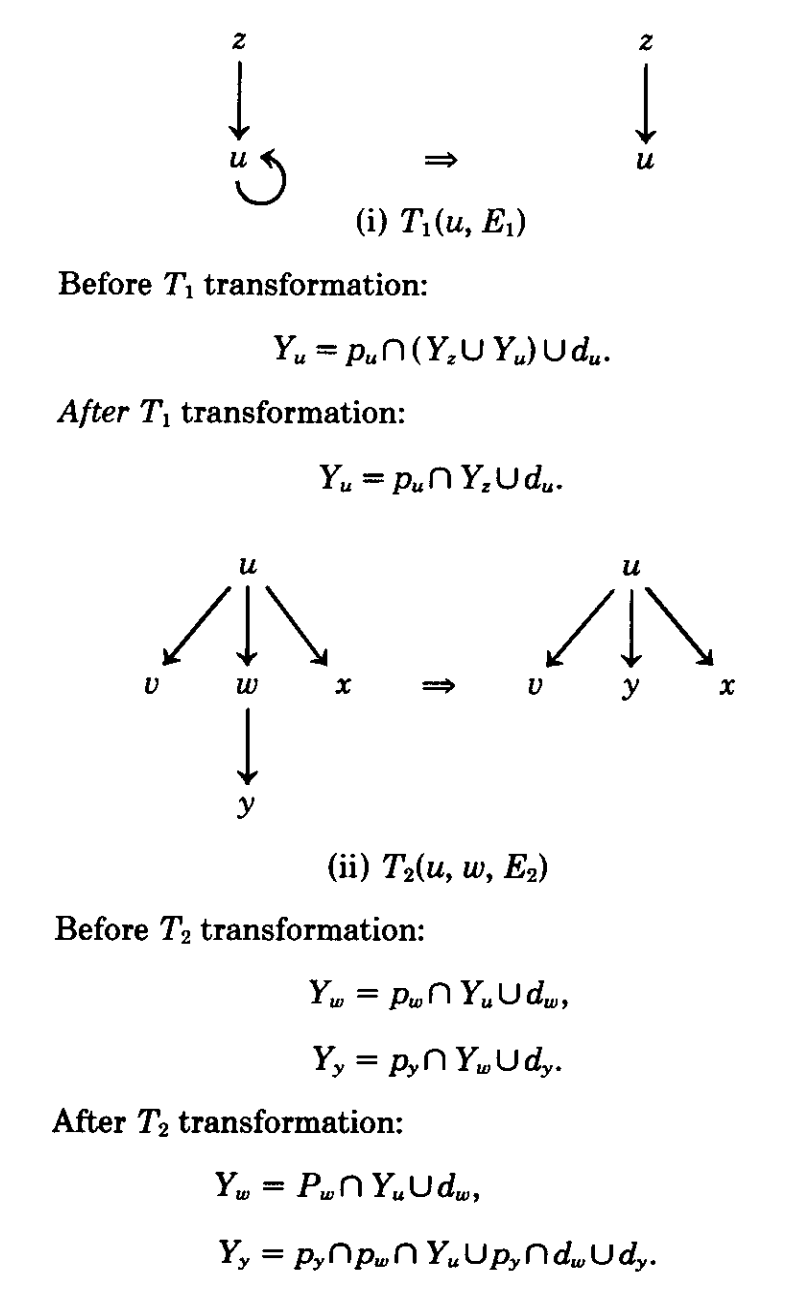
\includegraphics[width=0.8\textwidth]{transforms.png}
\end{figure}

Egy redukálható gráf egy \texttt{parse}-a (olvasata), $T_1$ és $T_2$ transzformációknak egy sorozata, mely az eredeti gráfot egyetlen csúcsú gráffá alakítja át. Egy-egy transzformációs lépést a transzformáció nevével, a redukálandó két csúccsal, illetve az őket összekötő éllel reprezentálunk. Fontos részlet, hogy egy \texttt{flow-graph} \texttt{parse}-a nem egyedi, függ a \texttt{flow-graph} reprezentációjától, attól például, hogy milyen sorrendben vizsgáljuk egy csúcsból kiinduló éleket. Lehetséges hogy egy csúcs több $T_1$ transzformációban is részt vesz, de egy él csak egy transzformációhoz tartozhat.

\begin{figure}[h]
\caption{Gráfok olvasata, transzfomációk sorozata. Forrás \cite{article}}
\centering
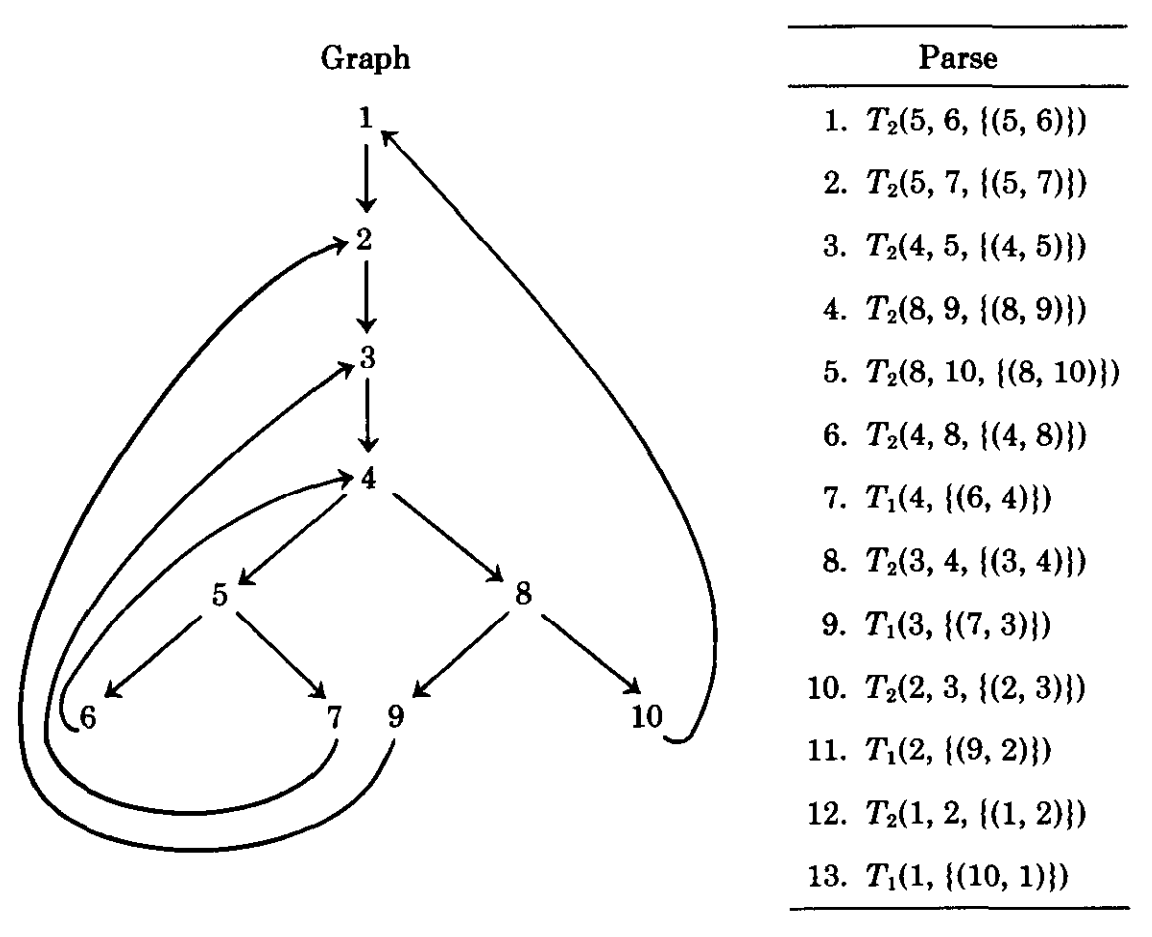
\includegraphics[width=0.8\textwidth]{parse.png}
\end{figure}

Az első fázis során olyan csúcsokat keres az algoritmus, melyek potenciálisan alanyát képezhetik a $T_2$ transzformációnak, illetve olyanokat melyek hurokélekkel rendelkeznek. A $T_2$ transzformáció olyan csúcsokra alkalmazható, melyeknek egyedi megelőzőjük van, vagyis amikor a csúcsnak megfeleltetett változót meghatározó függvény is csak egyetlen változó függvényeként felírható.

A $T_1$ transzformációt akkor használja az algoritmus, ha hurokélet talál az algoritmus. Ez a \texttt{data-flow} egyenletben megfelel annak hogy az egyenlet bal és jobb oldalán is megjelenik ugyanaz a változó. A A $T_1$ transzformáció kiküszöböli az egyenlet jobb oldaláról ezt a változót, az új rendszerhez illeszkedő \texttt{flow-graf}-ban pedig a hurokélet.

A második, redukciós fázisban megtörténik a függőségi szerepet betöltő \texttt{flow-graph}-ban a csúcsok összevonása $T_2$ esetében, illetve a csúcsok önmaguktól vett függőségeinek felszámolása $T_1$ esetében, viszont minden más művelet, mely olyan változókra vonatkozna, melyek még nem kerületek az adott transzformációk hatásaként egy régióba. Ezek kiértékelése késleltetett módon történik. Ez a késleltetés az algoritmus hatékonyságának az oka, mentesít attól hogy ugyanarra a változóra vonatkozóan többször számoljuk ki a redukciót.
Ahhoz hogy ezeket a közös számításokat késleltetve el tudja végezni az algoritmus egy különleges 2-3 kiegyensúlyozott erdőt használ.
A propagációs, harmadik lépésben már csak kezdőcsúcshoz tartozó változó értékének visszahelyettesítését kell elvégezni. Ennek a megoldásnak minden más változóhoz tartozó redukált egyenletébe visszahelyettesítve megkapjuk az egész probléma megoldását.

\section{Összegzés}

A \texttt{data-flow} analízis széles körben felhasznált módszer, melyet majdnem minden modern optimalizáló fordítóprogram felhasznál a fordított programkód javítására. Az analízis néhány klasszikus alkalmazása elegendőnek bizonyul számos optimalizációs lépés elvégzéséhez, és megvalósító algoritmusok is kis komplexitással meg tudják oldani a \texttt{data-flow} problémák előállítását általános esetben is. A redukciós stratégia alkalmazása népszerű az elemzést megvalósító alkalmazások körében, ezek az igényeknek megfelelően több hasonlóan jó komplexitással rendelkező eljárás közül választhatnak. 

\begin{thebibliography}{9}
\bibitem{book} 
Engineering a compiler second edition \\
Keith D. Cooper \& Linda Torczon
ISBN: 978-0-12-088478-0
 
\bibitem{article} 
Elimination Algorithms for Data Flow Analysis \\
BARBARA G. RYDER and MARVIN C. PAULL
ACM Computing Surveys, Vol. 18, No. 3, September 1986 
\end{thebibliography}

\end{document}